 \section{Results}

The resulting motion caused by one realization of the input disturbance is plotted in Figure~\ref{motionPlots}. It can be seen the disturbance is an impulse and the resulting motion is stable, settling back to the equilibrium point. Figure~\ref{ssEvolution} depicts the evolution of the maximum radius of the spot size during the simulation. The spot size radius is a positive definite quantity and the average spot size over the simulation time is the output metric.\\

\begin{figure}
	\centering
	\subfigure[]{
	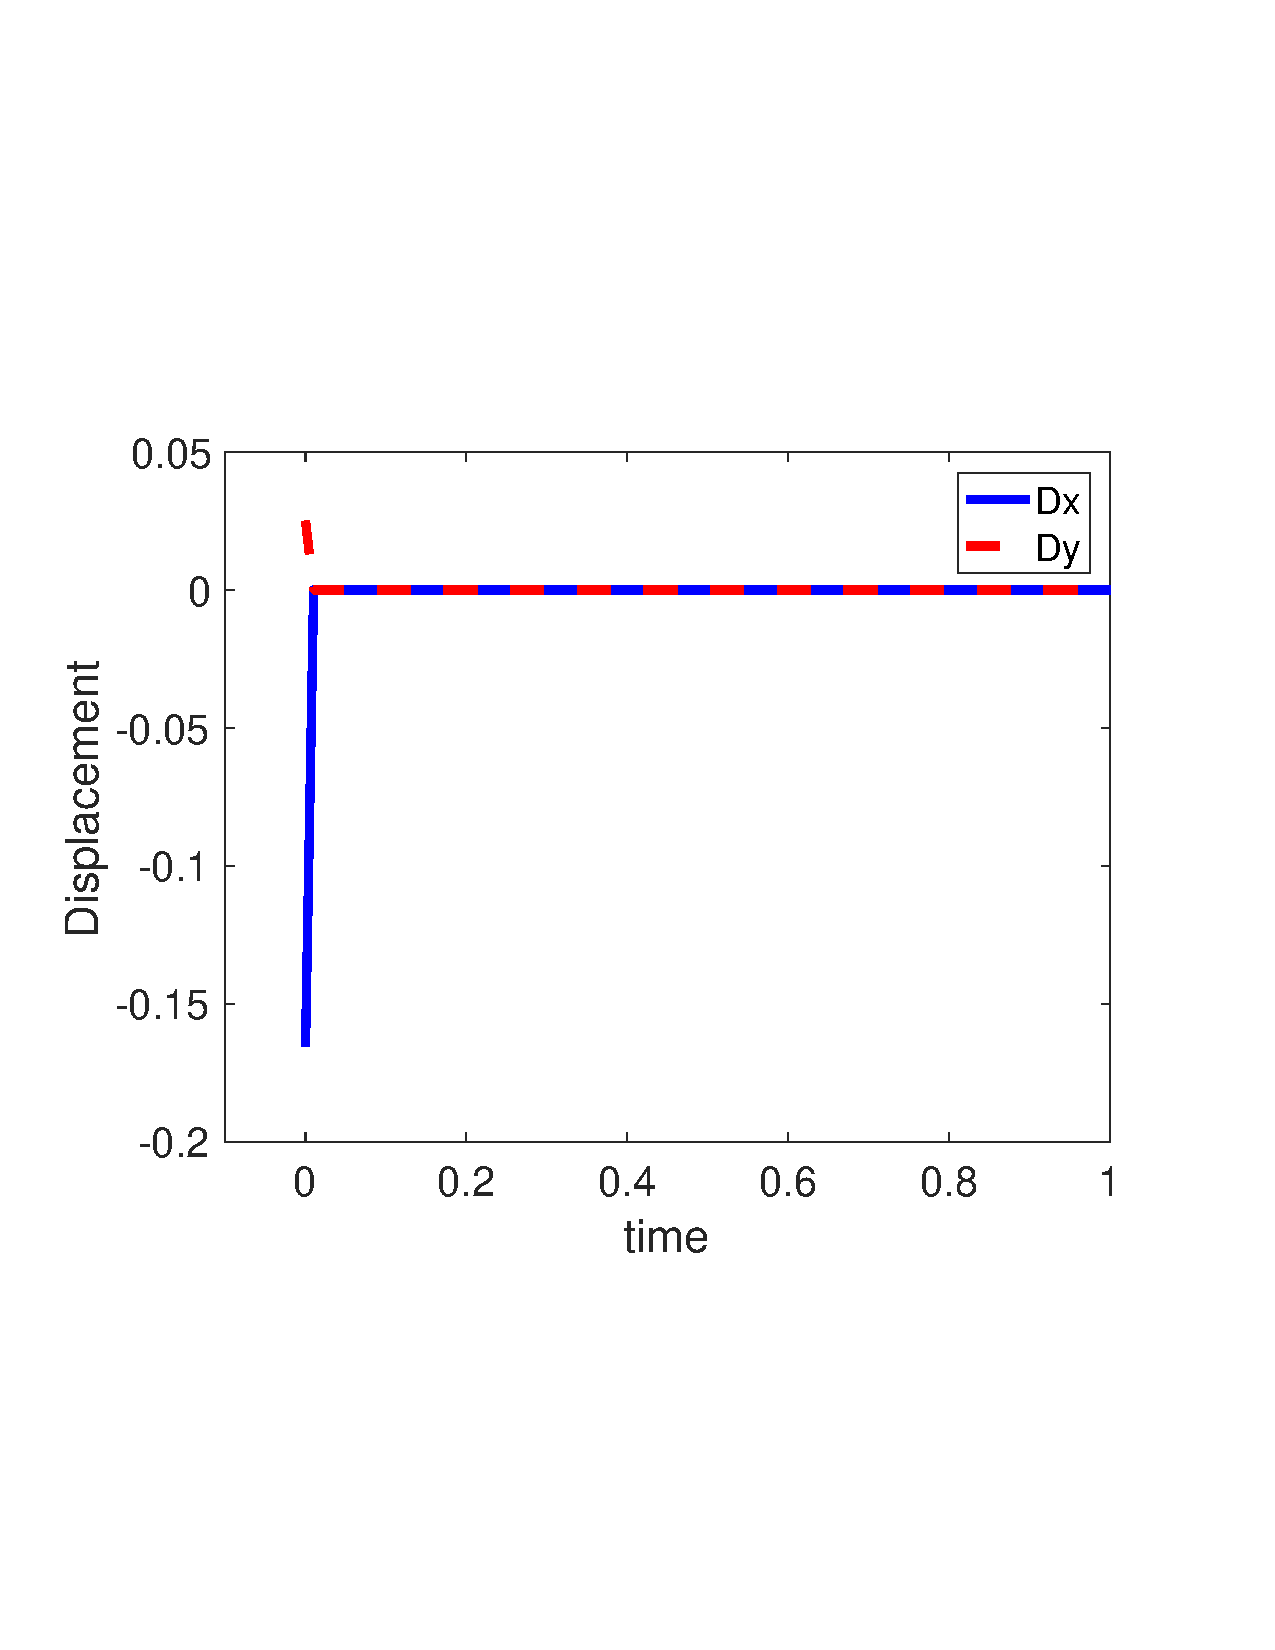
\includegraphics[width=0.45\textwidth,trim=0.8cm 6cm 2cm 6cm,clip]{Figures/Q5P1_real_Disturbance.pdf}}
	\subfigure[]{
	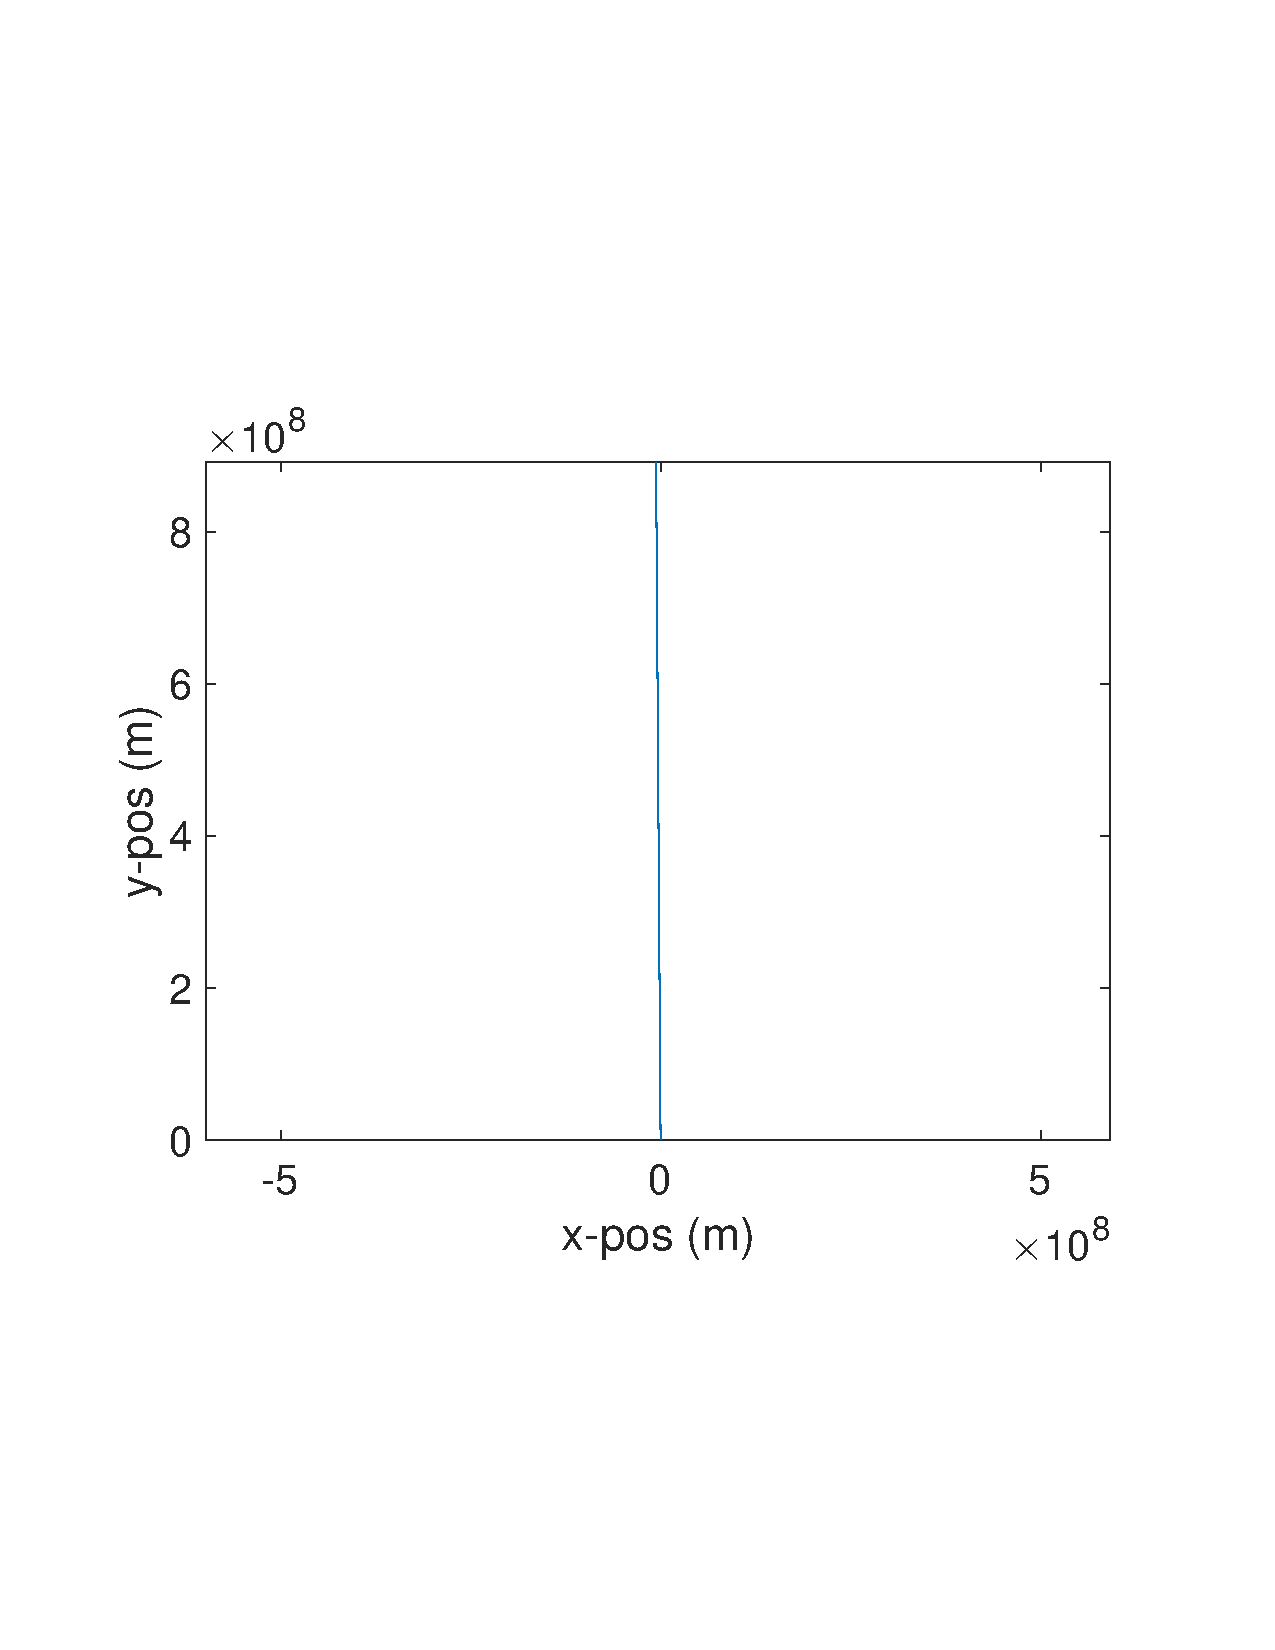
\includegraphics[width=0.45\textwidth,trim=0.8cm 6cm 2cm 6cm,clip]{Figures/Q5P1_real_CoM_Motion.pdf}}
	\subfigure[]{
	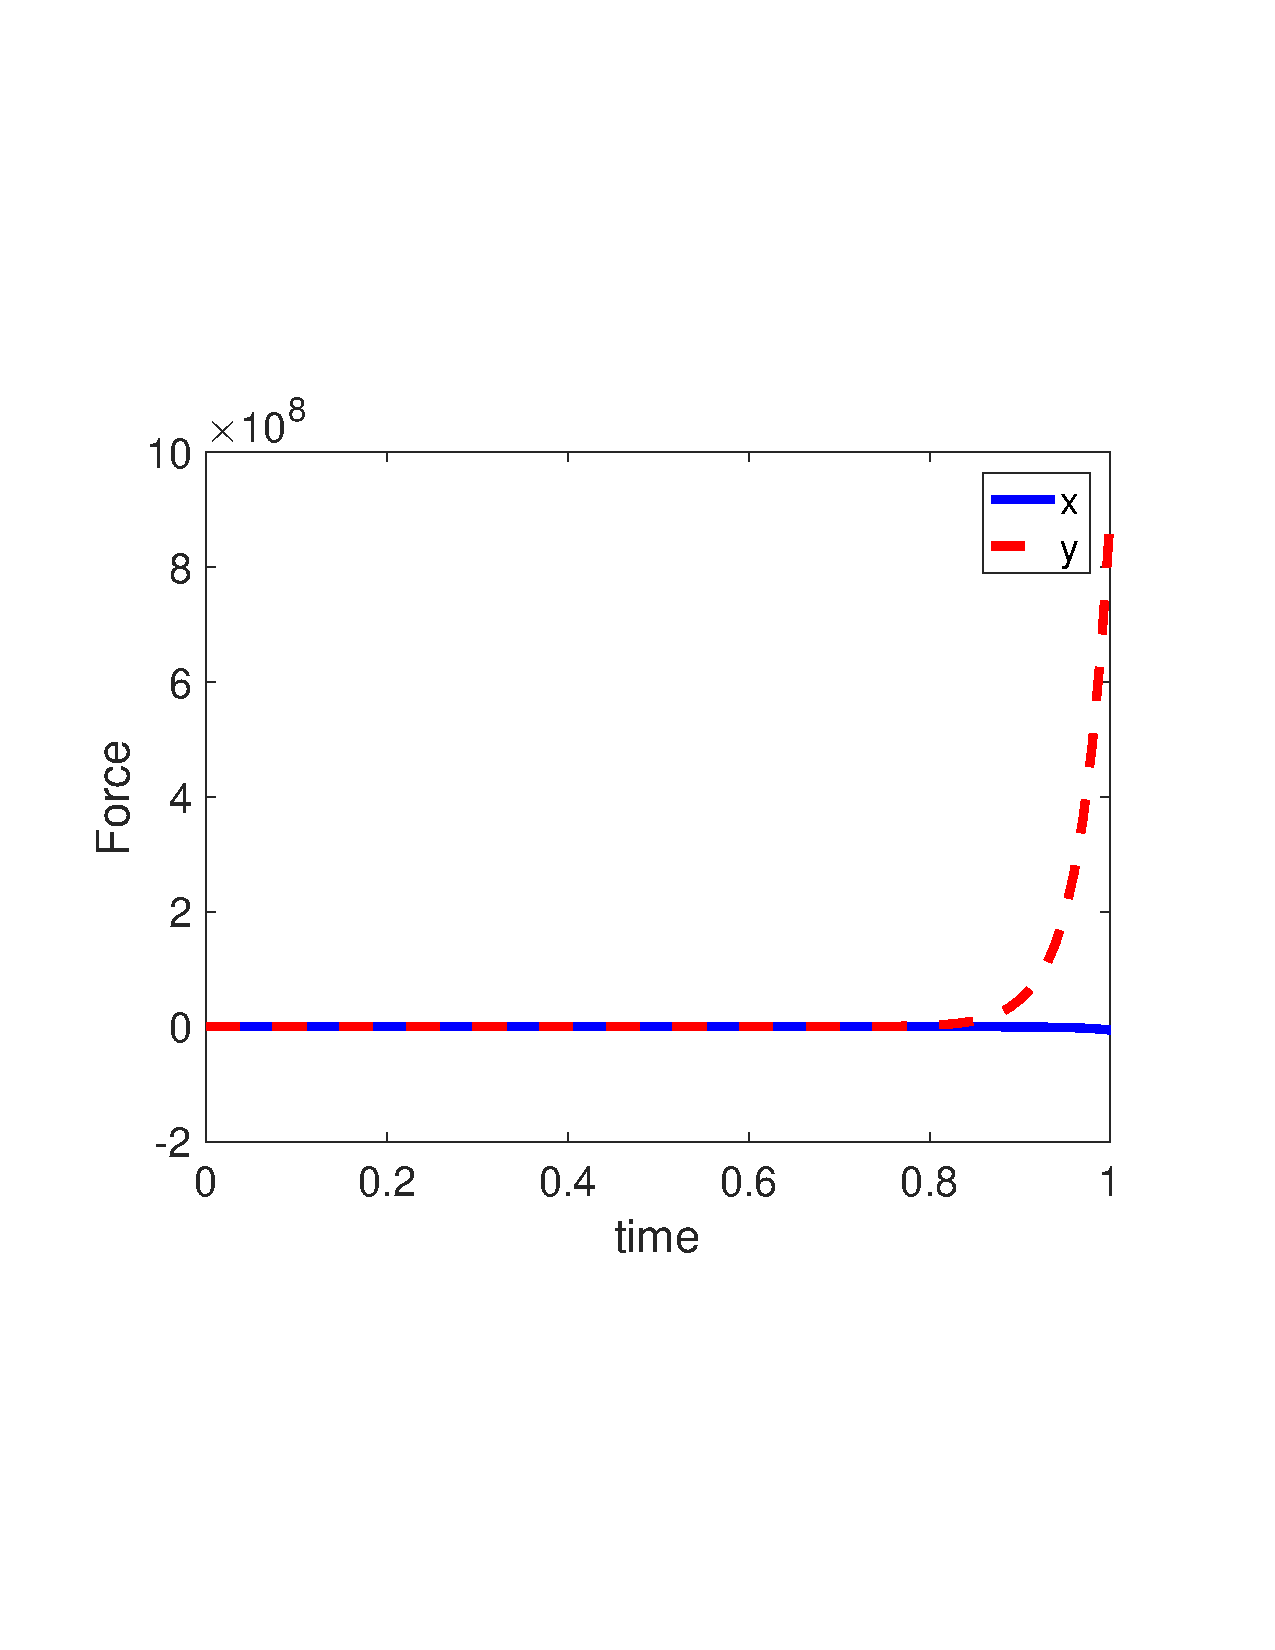
\includegraphics[width=0.45\textwidth,trim=0.8cm 6cm 2cm 6cm,clip]{Figures/Q5P1_real_CoM_LinDisp.pdf}}
	\subfigure[]{
	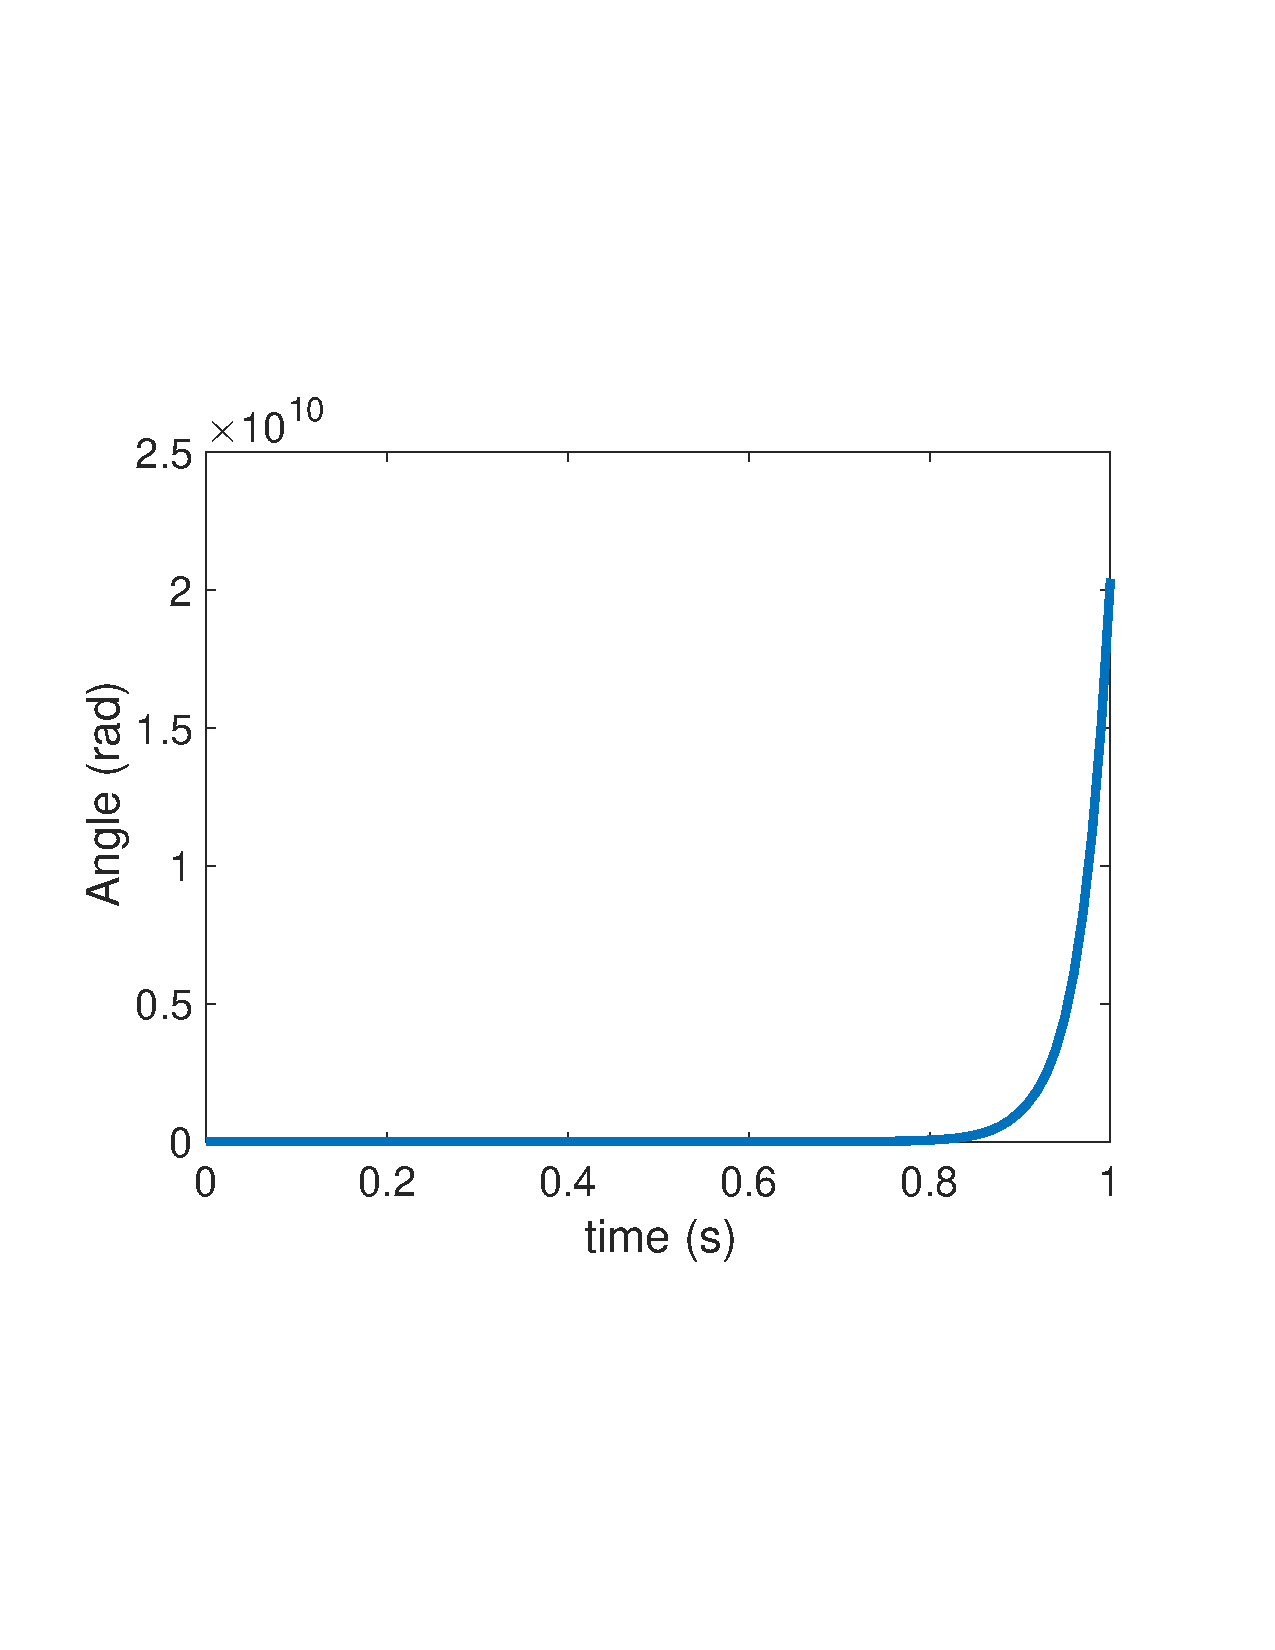
\includegraphics[width=0.45\textwidth,trim=0.8cm 6cm 2cm 6cm,clip]{Figures/Q5P1_real_CoM_AngDisp.pdf}}
	\caption{Dynamic responses to force disturbance. (a) Impulse force disturbance input at node \#2. (b) CoM motion. (c) CoM linear displacements. (d) Mirror angular displacement.}
	\label{motionPlots}
\end{figure}

\begin{figure}
	\centering
	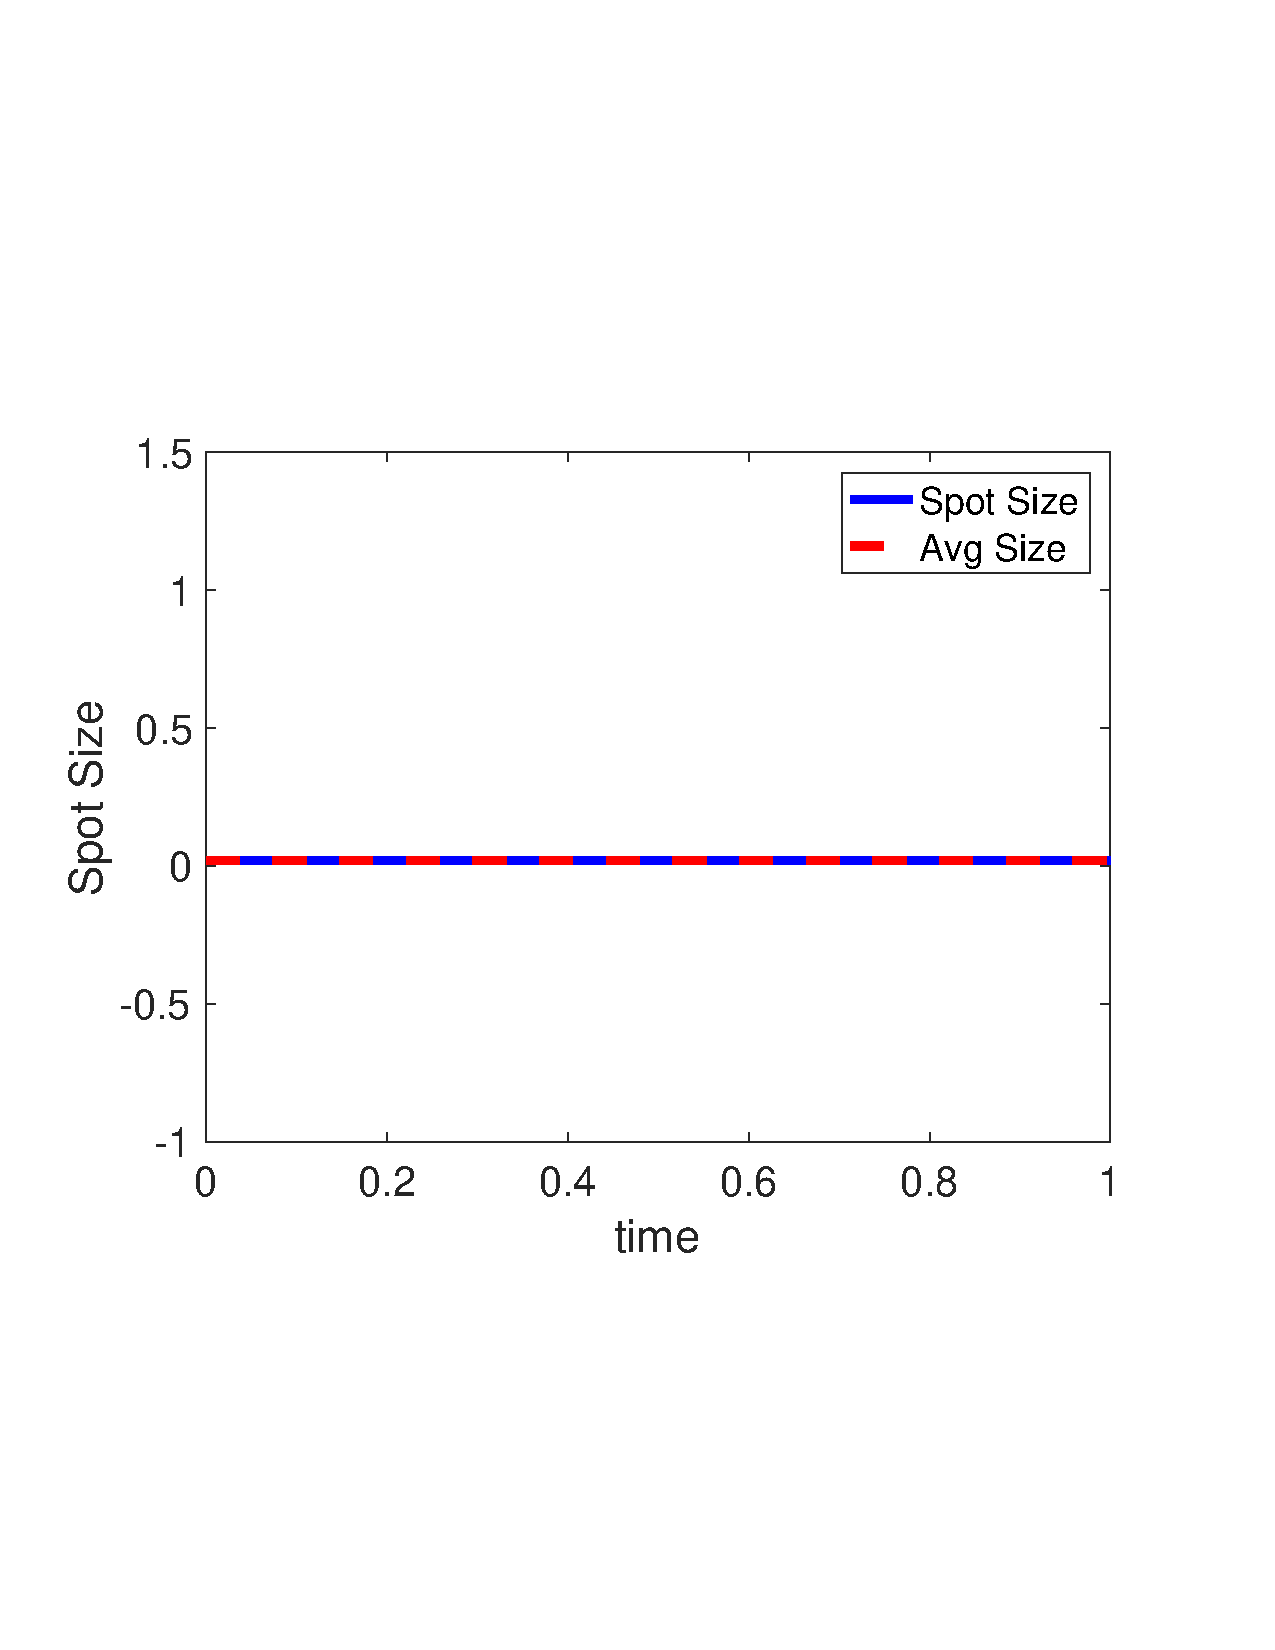
\includegraphics[width=0.65\textwidth,trim=1cm 6cm 2cm 6cm,clip]{Figures/Q5P1_real_SpotSizeEvolution.pdf}
	\caption{Detector plane maximum spot size radius evolution for a single realization.}
	\label{ssEvolution}
\end{figure}


MCS with random input disturbance realizations generate a sufficient number of output data sets for which the distribution parameters, $\mu_{out}$ and $\sigma_{out}$, are computed. These output distributions are then generated for varied user-supplied values of the input distribution parameters, $r_0$ and $\sigma_0$. Figures~\ref{distrel} are plots of the input to output statistics relationships. Analysis of these plots validates some intuition regarding the simulation. Figure~\ref{mu_v_r0} reveals a linear increase in the mean of the average spot size as the mean strength of the input disturbance is increased. Naturally, a larger disturbance generates a greater misalignment and poorer optical performance. Similarly, Figure~\ref{sigma_v_r0} shows a linear increase in the mean of input disturbance promotes an increase in the standard deviation of the average spot size. Figure~\ref{mu_v_sigma0} indicates that an increase in the standard deviation of the input disturbance does not noticeably change the mean of the average spot size except for zero-mean input. This observation suggests that the assumption of a Gaussian distribution of the output is appropriate because the distribution about the mean input mimics to the distribution about the mean output. Figure~\ref{sigma_v_sigma0} reveals an expected result in that the standard deviation about the mean output increases with the standard deviation of the input disturbance. \\

\begin{figure}
	\centering
	\subfigure[]{
	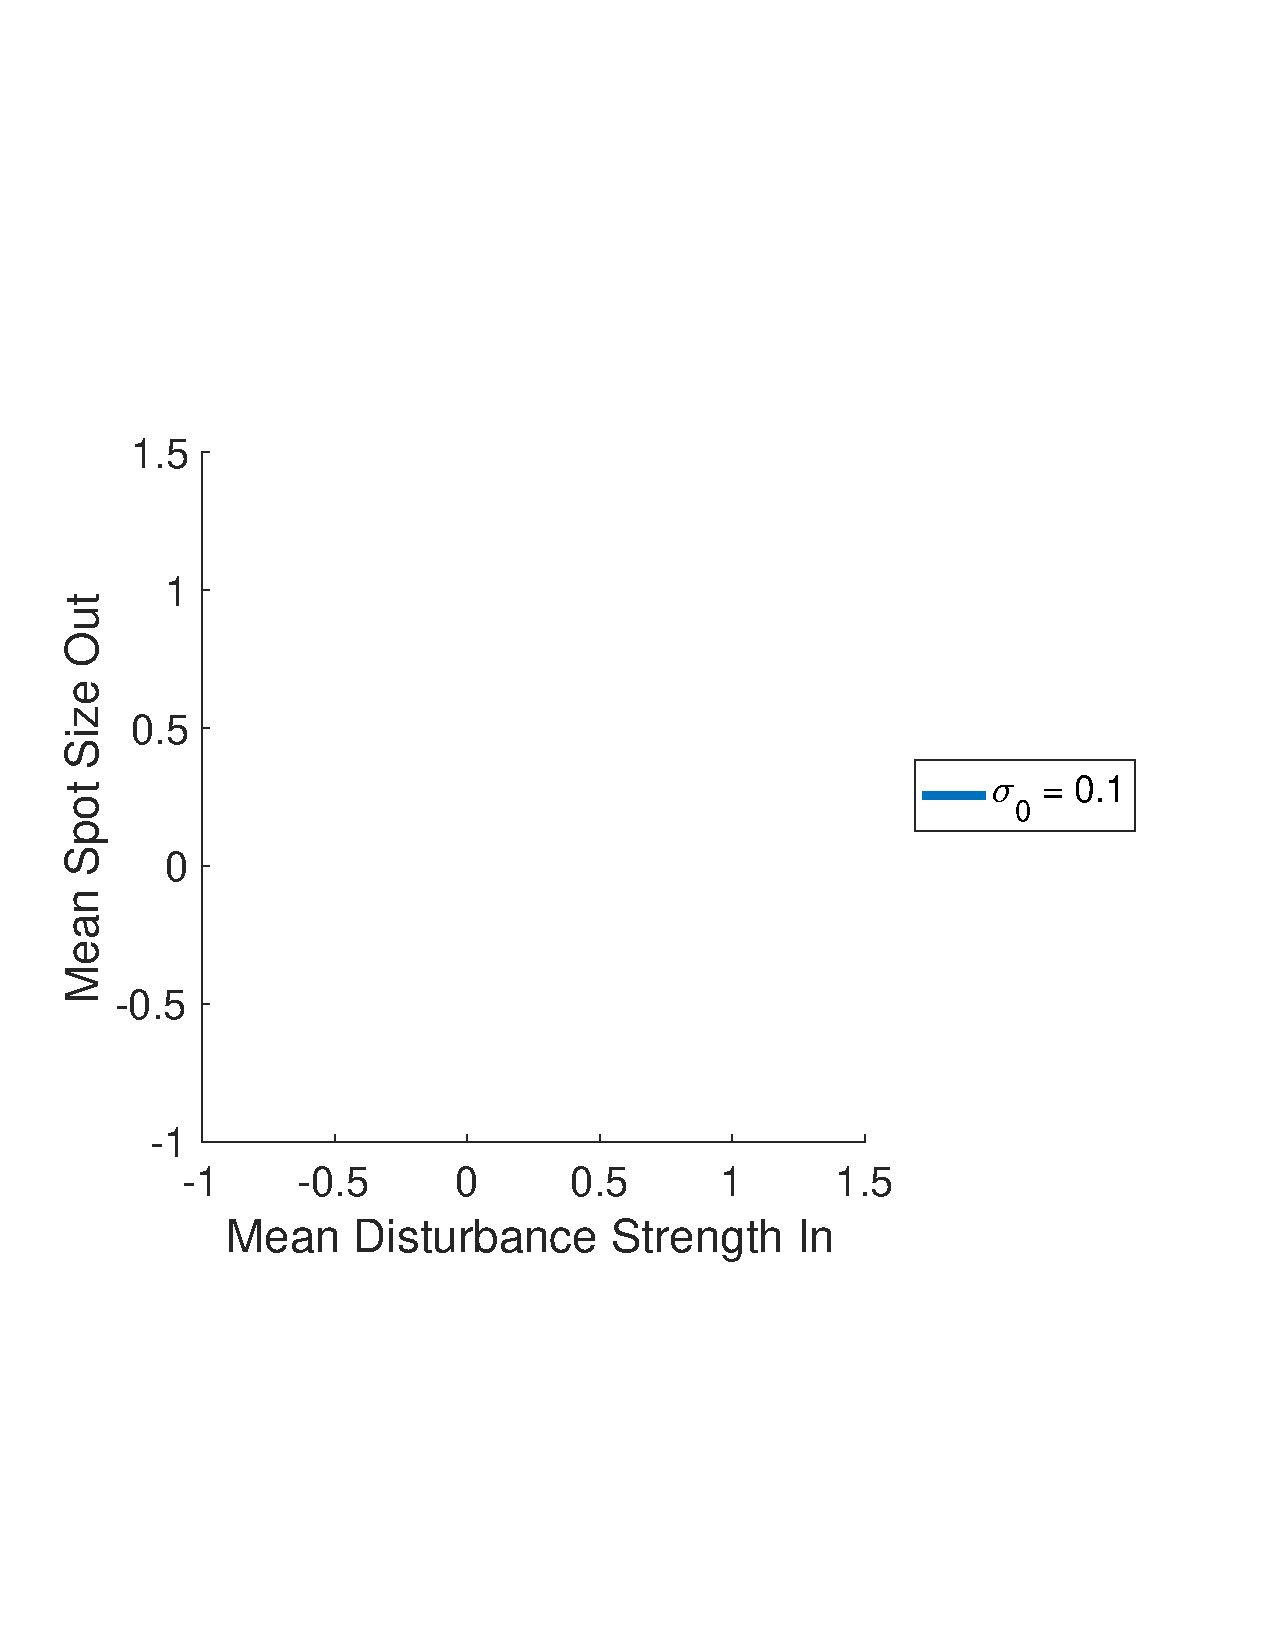
\includegraphics[width=0.45\textwidth,trim=0.8cm 6cm 2cm 6cm,clip]{Figures/Q5P1_stat_mu_v_r0.pdf}
	\label{mu_v_r0}}
	\subfigure[]{
	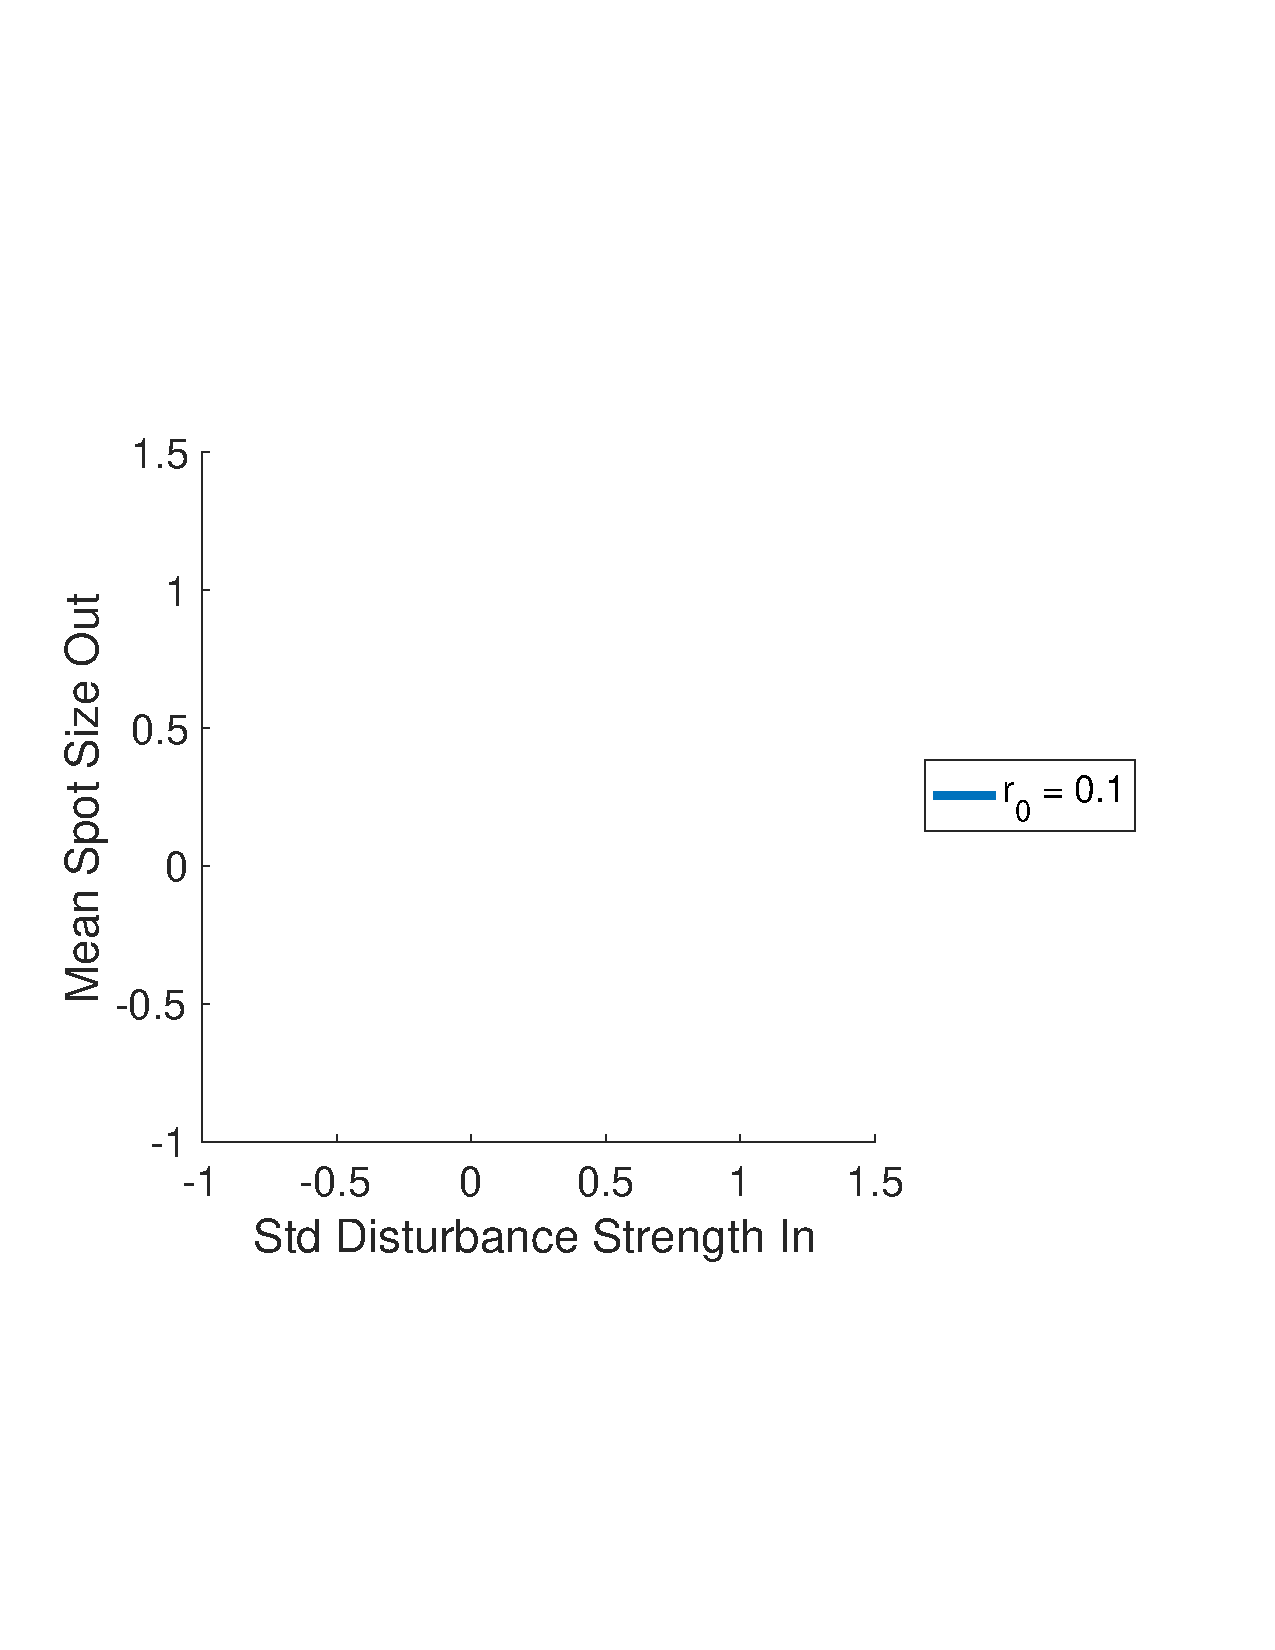
\includegraphics[width=0.45\textwidth,trim=0.8cm 6cm 2cm 6cm,clip]{Figures/Q5P1_stat_mu_v_sigma0.pdf}
	\label{mu_v_sigma0}}
	\subfigure[]{
	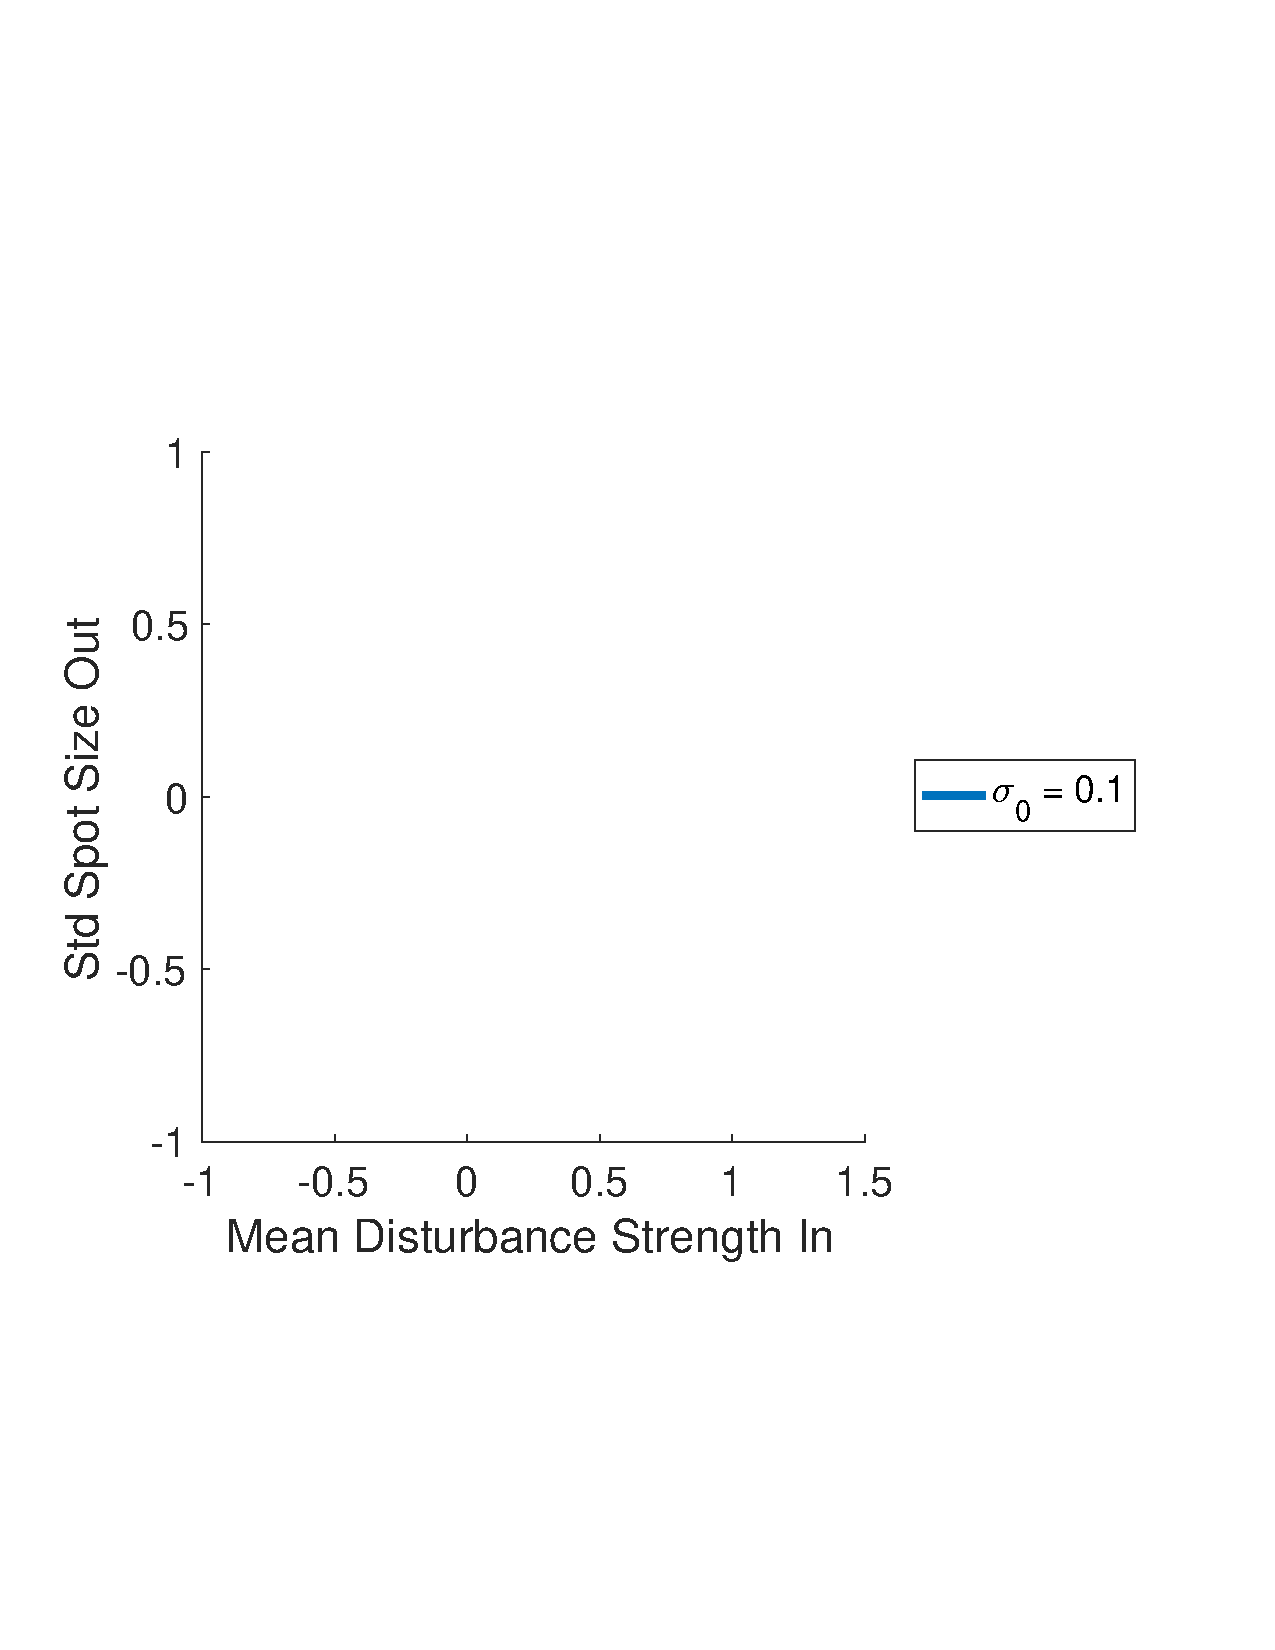
\includegraphics[width=0.45\textwidth,trim=0.8cm 6cm 2cm 6cm,clip]{Figures/Q5P1_stat_sigma_v_r0.pdf}
	\label{sigma_v_r0}}
	\subfigure[]{
	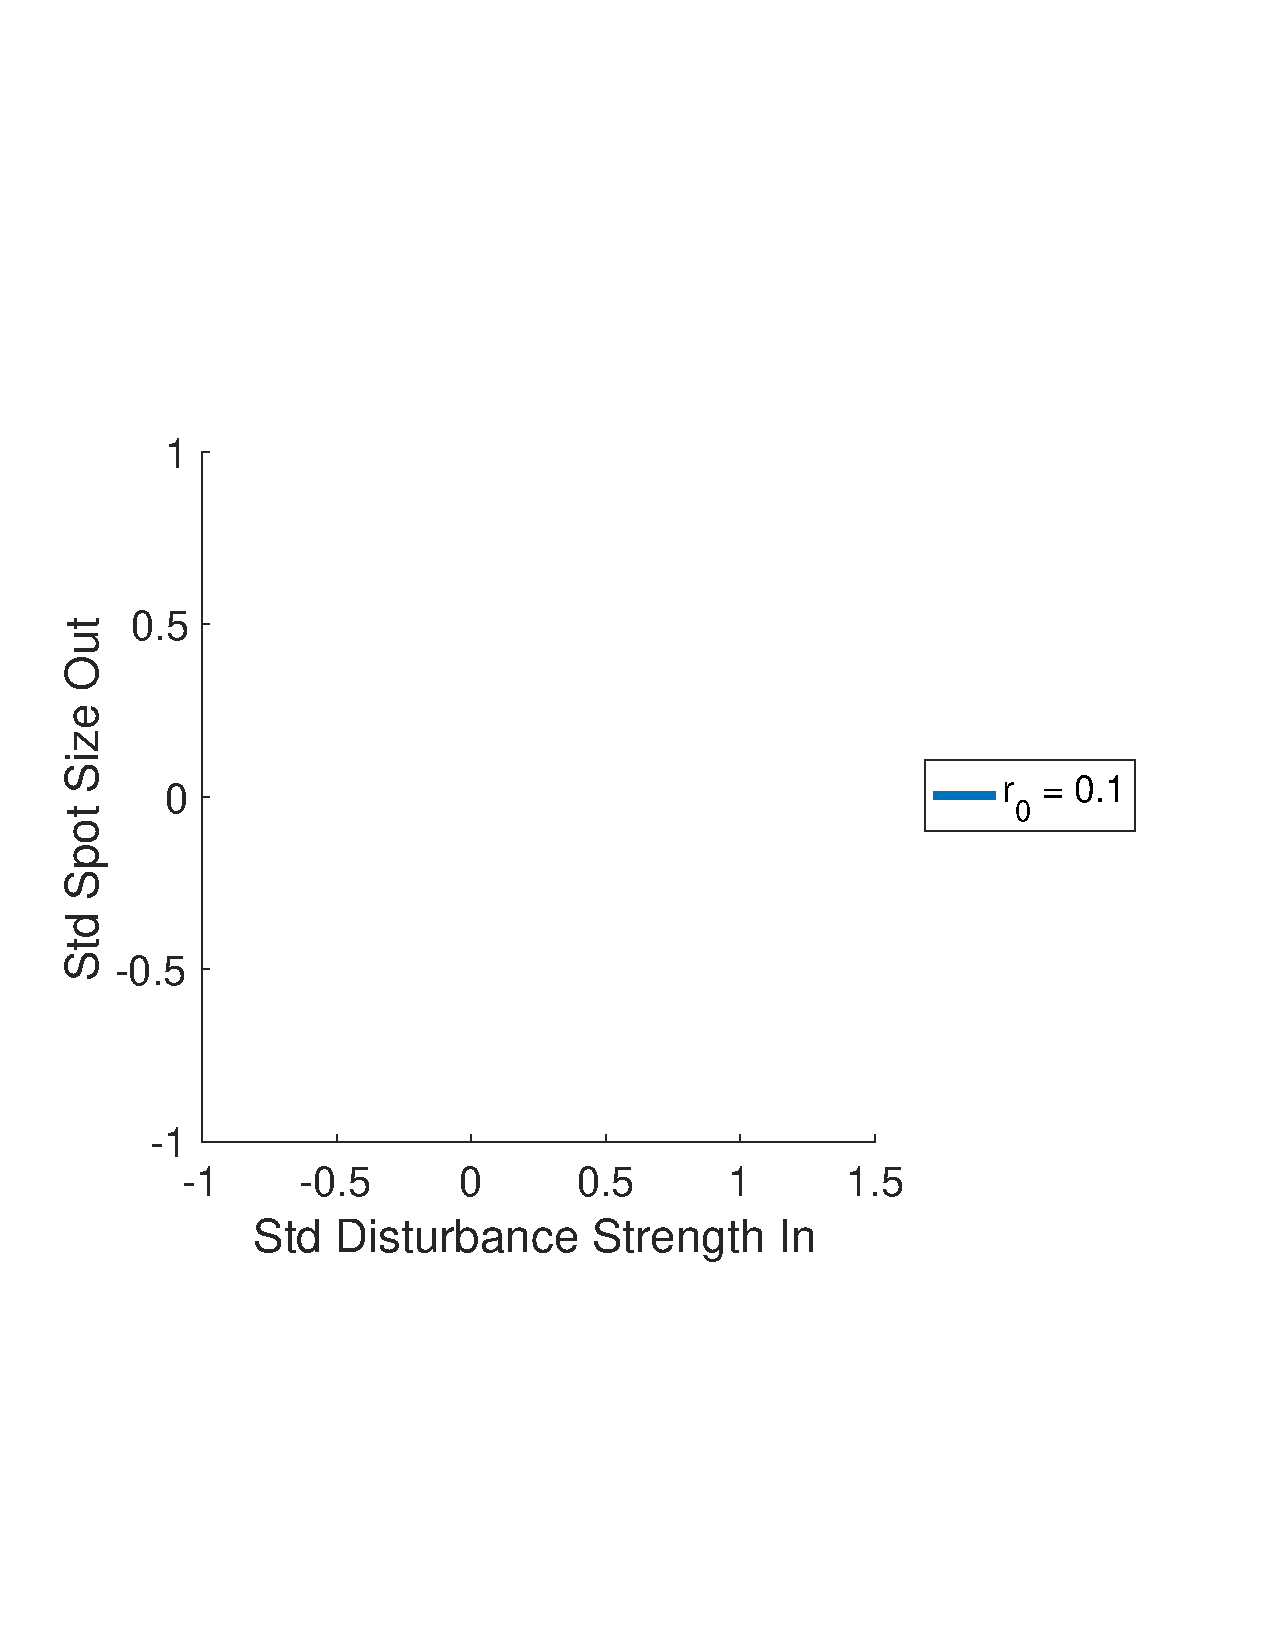
\includegraphics[width=0.45\textwidth,trim=0.8cm 6cm 2cm 6cm,clip]{Figures/Q5P1_stat_sigma_v_sigma0.pdf}
	\label{sigma_v_sigma0}}
	\caption{Distribution parameter relationships}
	\label{distrel}
\end{figure}

